%\textcolor{red}{\hrulefill \textsc{Unfinished Section}\hrulefill}  \\
The Muon Spectrometer (MS), located beyond the calorimeters is the outermost subdetector of ATLAS and is shown in Figure~\ref{fig:detector:muonspectrometer}.
It consists of three large air-core superconducting toroid systems (two end cap and one barrel) with eight coils each, providing a magnetic field of $\small\approx$ 0.5~T~\cite{ATLAS:2010xrj}.
The deflection of the muon trajectories in the bending plane of the magnetic field (the ``precision coordinate'') is measured via hits in three layers of monitored drift tube (MDT) precision chambers covering the region in pseudorapidity up to $|\eta|<$2.7.
In the innermost endcap wheels of the MS, cathode strip chambers (CSC) are used instead of MDTs in the region 2.0 $<|\eta|<$ 2.7~\cite{ATLAS:2010xrj}.
Three layers of resistive plate chambers (RPC) in the barrel ($|\eta|<$ 1.05) and 3–4 layers of thin gap chambers (TGC) in the endcaps (1.05$<|\eta|<$2.4) provide the muon trigger, and also measure the muon trajectory in the non-bending coordinate of the toroid magnets (the ``second coordinate'')~\cite{ATLAS:2010xrj}.
In the Phase-I upgrade, during the second long shutdown (LS2), the Small Wheels will be replaced by the New Small Wheels (NSW) that use a small-strip TGC and Micro-Mesh Gaseous Structure chambers used for both triggering and precision tracking~\cite{ATLAS:2010xrj}.
\begin{figure}[h]
\makebox[\textwidth][c]{
    \centering
    \begin{subfigure}[b]{0.45\textwidth}
      \centering
      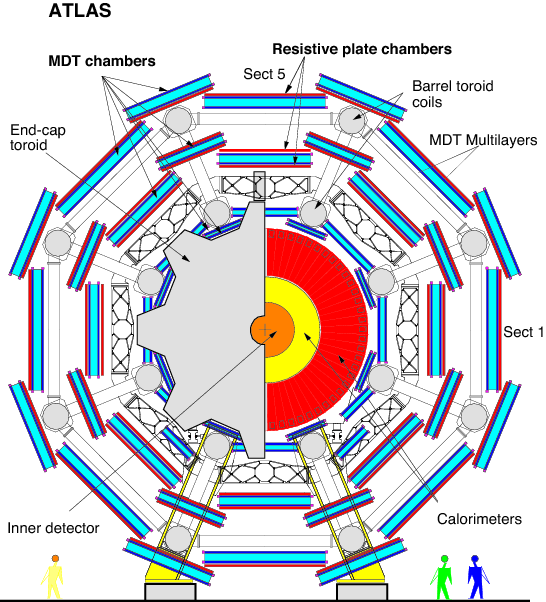
\includegraphics[width=1.0\textwidth]{figs/detector/MuonSpec1.png}
      \caption{}
      \label{fig:detector:muonspec1}
    \end{subfigure}
    \hfill
    \begin{subfigure}[b]{0.70\textwidth}
      \centering
      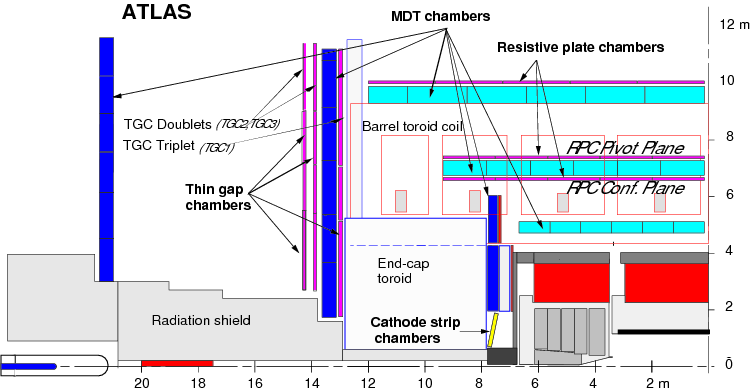
\includegraphics[width=1.0\textwidth]{figs/detector/MuonSpec2.png}
      \caption{}
      \label{fig:detector:muonspec2}
    \end{subfigure}
}
  \caption[The muon spectrometer system.]
          {(a) A cross sectional view in the r-$\phi$ plane of the barrel layout of the muon spectrometer as well as the view (b) in the $\eta$-z plane depicting the MS endcap systems with the two outermost TGC systems also being known as the ``wheels''~\cite{ATLAS:2010xrj}.}
      \label{fig:detector:muonspectrometer}
\end{figure}
